% !TeX spellcheck = de_DE
\documentclass{uebung_cs}
\usepackage{algo221}
\uebung{7}{}{}
\blattname{Übungen zu Woche 7: Hartnäckigkeit I}

\usepackage[ruled]{algorithm2e}

%%%%%%%%%%%%%%%%%%%%%%%%%%%%%%%%%%%%%%%%%%%%%%%%%%%%%%%%%%%%%%%%%%%%%%%%%%%%
\begin{document}

Das Übungsblatt enthält alle empfohlenen Lernaktivitäten für die aktuelle Woche.

\begin{itemize}
\item \textbf{Heimarbeit bis Montag 17:00.}
    \begin{itemize}
    \item 
    Schau die Videos an und lies die Buchkapitel.
    \item Bearbeite die \emoji{seedling}-Aufgabe in \href{https://moodle.studiumdigitale.uni-frankfurt.de/moodle/course/view.php?id=2241}{Moodle}. (Feste Abgabefrist!)
    \item Lese den Aufgabentext aller Übungsaufgaben.
    \end{itemize}
\item \textbf{Heimarbeit.} Bearbeite die Übungsaufgaben soweit möglich. Probier zumindest alle mal!
\item \textbf{Dienstag/Donnerstag.}
\begin{itemize}
    \item \textbf{8:00--8:15.} Besprechung im Hörsaal.
    \item \textbf{8:15--9:15.} Bearbeite jetzt die Übungen, die du noch nicht lösen konntest. Sprich mit anderen Studis! Frag das Vorlesungsteam um Hilfe!
    \item \textbf{9:15--9:45.} Lösungsspaziergang zu den Aufgaben für heute.
\end{itemize}

\item \textbf{Heimarbeit bis Freitag, den 03.12., 17:00.} Gib deine Lösungen zu der \emoji{star}-Aufgabe von diesem Übungsblatt in \href{https://moodle.studiumdigitale.uni-frankfurt.de/moodle/course/view.php?id=2241}{Moodle} ab. (Feste Abgabefrist!)
\end{itemize}

\section*{Dienstag}

\begin{aufgabe}[Schaltkreise]
	% Eigenkreation
	In der Vorlesung haben wir eine Reduktion von \textsc{CircuitSat} auf \textsc{3SAT} gesehen. Gegeben sei folgender Schaltkreis:
	
	\begin{figure}[ht]
		\begin{center}
			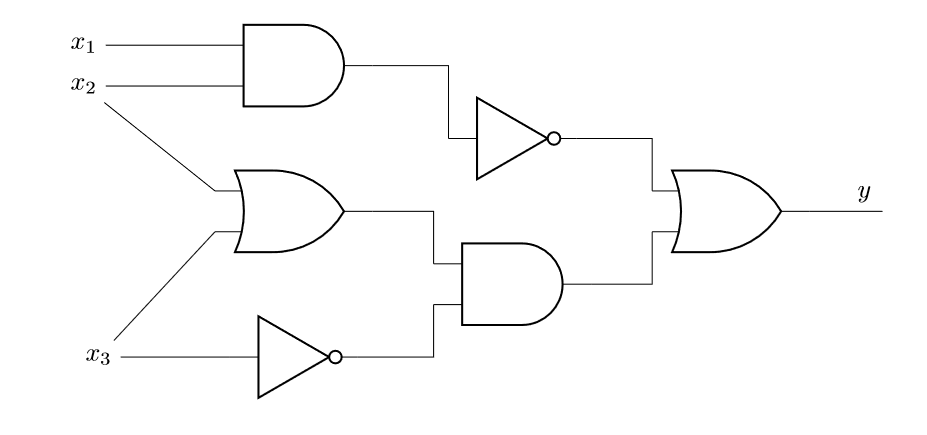
\includegraphics[scale=0.5]{schaltkreis}
		\end{center}
	\end{figure}
	% \begin{center}
	% \begin{circuitikz} 
	% \ctikzset{logic ports=ieee}
    % 	\draw
	% 	(0,2)  node[and port] (and_1) {}
	% 	(0,0)  node[or port]  (or_1)  {}
	% 	(0,-2) node[not port] (not_1) {}
	% 	(3,1)  node[not port] (not_2) {}
	% 	(3,-1) node[and port] (and_2) {}
	% 	(6,0)  node[or port]  (or_2)  {}
	% 	(and_1.out) -| (not_2.in)
	% 	(or_1.out)  -| (and_2.in 1)
	% 	(not_1.out) -| (and_2.in 2)
	% 	(and_2.out) -| (or_2.in 2)
	% 	(not_2.out) -| (or_2.in 1)
	% 	(or_2.out) -- ++(1,0) node[near end,above]{$y$}
		
	% 	(and_1.in 1) -- ++(-1.5,0)node[left](In1){$x_1$}
	% 	(and_1.in 2) -- ++(-1.5,0)node[left](In2){$x_2$}
	% 	(or_1.in 1) -- (In2)
	% 	(not_1.in) -- ++(-1.5,0)node[left](In3){$x_3$}
	% 	(or_1.in 2) -- (In3);
	% \end{circuitikz}
	% \end{center}
	
	Welche \textsc{3CNF} Formel gibt die Reduktion aus, wenn die Eingabe aus dem dargestellten Schaltkreis besteht?\\
\end{aufgabe}

\begin{aufgabe}[DNF Erfüllbarkeit]
	% Erickson, Chapter 12, Exercise 3
	Eine aussagenlogische Formel ist in \textit{disjunktiver Normalform} (DNF), wenn sie eine Disjunktion (\textsc{Or}) von Konjunktionstermen (\textsc{And}) ist. Ein Beispiel für eine DNF ist:
	$$(\overline{x} \wedge y \wedge \overline{z}) \vee (y \wedge z) \vee (x \wedge \overline{y} \wedge \overline{z}).$$
	Gegeben ist eine aussagenlogische Formel in disjunktiver Normalform. DNF-\textsc{Sat} entscheidet, ob diese Funktion erfüllbar ist.
	\begin{enumerate}
		\item Beschreibe einen Algorithmus, der DNF-\textsc{Sat} in Polynomialzeit  löst.
		\item Was ist der Fehler im folgenden Argument, in dem $\P = \NP$ gezeigt wird?
		\begin{quote}
			Angenommen, wir haben eine aussagenlogische Formel in konjunktiver Normalform mit höchstens 3 Literalen pro Klausel. Wir wollen herausfinden, ob diese Funktion erfüllbar ist. Wir können das Distributivgesetz für Boolesche Operationen verwenden, um eine äquivalente Formel in disjunktiver Normalform zu konstruieren. Zum Beispiel:
			$$(x \vee y \vee \overline{z}) \wedge (\overline{x} \vee \overline{y}) \Leftrightarrow (x \wedge \overline{y}) \vee (y \wedge \overline{x}) \vee (\overline{z} \wedge \overline{x}) \vee (\overline{z} \wedge \overline{y}).$$
			Nun können wir den Algorithmus aus Aufgabenteil a) verwenden, um in Polynomialzeit herauszufinden, ob die entstandene DNF erfüllbar ist. Wir haben also \textsc{3Sat} in Polynomialzeit gelöst! Da \textsc{3Sat} $\NP$-hart ist, gilt $\P = \NP$!	
		\end{quote}
	\end{enumerate}	 
\end{aufgabe}

\begin{aufgabe}[Perfektes Matching]\
	% https://courses.engr.illinois.edu/cs374/fa2021/A/labs/lab12.pdf - Exercise 1
	Sei $G = (V,E)$ ein ungerichteter Graph. Eine Teilmenge $M \subseteq E$ ist ein \textit{Matching}, wenn keine zwei Kanten aus $M$ mit demselben Knoten verbunden sind. Ein Matching ist \textit{perfekt}, wenn jeder Knoten $v \in V$ zu einer Kante $m \in M$ inzident ist. Eine andere mögliche Definition betrachtet die Größe des Matchings: $M$ ist perfekt, wenn $|M| = |V|/2$ gilt. Wir definieren das \textsc{PerfektesMatching}-Problem:
	\begin{quote}
		\textsc{PerfektesMatching}:\\
		Gegeben sei ein ungerichteter Graph $G = (V,E)$. Existiert in $G$ ein perfektes Matching?
	\end{quote}
	Dieses Problem kann in Polynomialzeit gelöst werden. Das ist ein fundamentales Ergebnis der kombinatorischen Optimisierung mit vielen Anwendungen in Theorie und Praxis. Es stellt sich heraus, dass das \textsc{PerfektesMatching}-Problem auf bipartiten Graphen einfacher zu lösen ist. Ein Graph $G = (V,E)$ ist \textit{bipartit}, wenn die Menge der Knoten $V$ auf zwei Teilmengen~$L$ und~$R$ verteilt werden können, sodass alle Kanten zwischen $L$ und $R$ liegen. In anderen Worten: $L$ und $R$ sind unabhängige Knotenmengen (Independent Set). Im Folgenden ist ein Algorithmus vorgeschlagen, der allgemeine Graphen auf bipartite Graphen reduziert:
	\begin{quote}
		\textsc{ReduceGraph}:\\
		Gegeben sei ein ungerichteter Graph $G = (V,E)$. Erstelle daraus einen bipartiten Graphen $H = (V \times \{1,2\},E_H)$ wie folgt:\\
		Jeder Knoten $u \in V$ wird zu zwei Kopien $(u,1)$ und $(u,2)$. Dabei ist \[V_1 = \{(u,1)\,|\,u\in V\}\] eine Seite und \[V_2 = \{(u,2)\,|\,u\in V\}\] die andere Seite des bipartiten Graphen. Sei \[E_H = \{\{(u,1),(v,2)\}\,|\,\{u,v\} \in E\}\,.\] In anderen Worten: Wenn $\{u,v\} \in E$, fügen wir eine Kante zwischen $(u,1)$ und $(v,2)$ ein. Beachte, dass es keine Eigenschleifen in $G$ gibt und es dadurch in $H$ für alle $u \in V$ keine Kante  $\{(u,1),(u,2)\}$ geben kann.
	\end{quote}
	Ist die vorgeschlagene Reduktion korrekt? Um das herauszufinden müssen wir überprüfen, ob $H$ nur genau dann ein perfektes Matching hat, wenn $G$ eins hat.
	\begin{enumerate}
		\item Zeige: Wenn $G$ ein perfektes Matching hat, dann hat auch $H$ eins.
		\item Sei $G$ der vollständige Graph mit $3$ Knoten, also ein Dreieck. Zeige: $G$ hat kein perfektes Matching, aber $H$ hat eins.
		\item Erweitere das Beispiel aus der vorherigen Teilaufgabe: Konstruiere einen Graphen $G$ mit einer geraden Anzahl an Knoten, sodass $G$ kein perfektes Matching hat, $H$ aber schon.
	\end{enumerate}
	Damit ist die Reduktion inkorrekt, obwohl eine Richtung wahr ist.
\end{aufgabe}

\begin{aufgabe}[Independent Set]\
	% https://courses.engr.illinois.edu/cs374/fa2021/A/labs/lab12.pdf - Exercise 2
	Ein \emph{Independent Set} in einem Graphen $G = (V,E)$ ist eine Teilmenge $S \subseteq V$, sodass keine zwei Knoten $u,v \in S$ durch eine Kante $\{u,v\} \in E$ verbunden sind. Du hast eine magische Blackbox, die auf wundersame Art und Weise das folgende Entscheidungsproblem in Polynomialzeit beantwortet:
	\begin{itemize}[topsep=0.21cm, leftmargin=1.2cm]
		\item \textsc{Input}: Ein ungerichteter Graph $G$ und eine Zahl $k \in \N$.
		\item \textsc{Output}: \textsc{True}, wenn $G$ ein Independent Set der Größe $k$ besitzt, sonst \textsc{False}.
	\end{itemize}
	\begin{enumerate}
		\item Benutze die Blackbox, um einen Algorithmus zu beschreiben, der folgendes Optimisierungsproblem in Polynomialzeit löst:
		
		\begin{itemize}[topsep=0.21cm, leftmargin=1.2cm]
			\item \textsc{Input}: Ein ungerichteter Graph $G$.
			\item \textsc{Output}: Die Größe des größten Independent Set in $G$.
		\end{itemize}
		\item Benutze die Blackbox, um einen Algorithmus zu beschreiben, der folgendes Suchproblem in Polynomialzeit löst:
		
		\begin{itemize}[topsep=0.21cm, leftmargin=1.2cm]
			\item \textsc{Input}: Ein ungerichteter Graph $G$.
			\item \textsc{Output}: Ein Independent Set in $G$ mit maximaler Größe.
		\end{itemize}
	\end{enumerate}
\end{aufgabe}

\section*{Donnerstag}

\begin{aufgabe}[NP]\
	% KT - Exercise 8.1
	Entscheide für die beiden folgenden Fragen, welche der Antworten \glqq Ja\grqq{}, \glqq Nein\grqq{} oder \glqq Unbekannt, da es $\P = \NP$ beantworten würde\grqq{} zutrifft. Erkläre kurz, warum du dich für deine Antwort entschieden hast.

	\begin{quote}
		\textsc{IntervalScheduling}: \\
		Sei eine Menge von Intervallen auf einer Zeitleiste und eine Schranke $k$ gegeben. Enthält diese Menge an Intervallen eine Teilmenge von sich nicht überschneidenden Intervallen der Größe mindestens $k$?
	\end{quote}
	
	Im Folgenden schreiben wir $A \leq_p B$, wenn es eine Polynomialzeit-Reduktion gibt, die das Problem $A$ auf das Problem $B$ reduziert. Das heißt, das Problem $A$ soll in Polynomialzeit gelöst werden, falls es einen magischen Algorithmus gibt, der $B$ in Polynomialzeit löst.
	\begin{enumerate}
		\item Gilt \textsc{IntervalScheduling} $\leq_p$ \textsc{VertexCover}?
		\item Gilt \textsc{IndependentSet} $\leq_p$ \textsc{IntervalScheduling}?
	\end{enumerate}
\end{aufgabe}


\begin{aufgabe}[Kundenanalyse]\
	% KT - Exercise 8.2
	Zur Analyse des Kundenverhaltens benutzen Geschäfte oftmals ein zweidimensionales Array $A$, wo die Zeilen die Kunden und die Spalten die verkauften Produkte enthalten. Ein Eintrag $A[i,j]$ gibt an, welche Menge von Produkt $j$ der Kunde $i$ gekauft hat, so hat Chelsea im folgenden Beispiel siebenmal Katzenstreu gekauft.
	
	\begin{center}
	\begin{tabular}{l c c c c}
	\hline 
	& Waschmittel & Bier & Windeln & Katzenstreu \\ 
	\hline 
	Raj & 0 & 6 & 0 & 3 \\ 
	Alanis & 2 & 3 & 0 & 0 \\ 
	Chelsea & 0 & 0 & 0 & 7 \\ 
	\hline 
	\end{tabular} 
	\end{center}
	
	Ein Geschäft möchte nun eine \textit{diverse} Teilmenge der Kunden finden, weil das nützlich sein kann, um Marktforschung zu betreiben. Eine Teilmenge $S$ der Kunden heißt \textit{divers}, wenn keine zwei Kunden aus $S$ dieselben Produkte gekauft haben. Mit anderen Worten gibt es für jedes Produkt nur genau einen Kunden aus $S$, der es gekauft hat. Das lässt sich als das Problem \textsc{DiverseTeilmenge} formulieren.
	\begin{quote}
		\textsc{DiverseTeilmenge}:\\
		Seien ein $n \times m$ Array $A$, wie oben definiert, und eine Zahl $k$ mit $k \leq n$ gegeben. Gibt es eine \textit{diverse} Teilmenge $S$ der Kunden mit $|S| \geq k$?
	\end{quote}
	Zeige, dass \textsc{DiverseTeilmenge} \NP-vollständig ist.
\end{aufgabe}    

% \begin{aufgabe}[Feriencamp]
% 	% KT - Exercise 8.3
% 	Bei der Organisation eines Feriencamps wirst du mit dem Problem \textsc{EffizientesRekrutieren} konfrontiert.
% 	\begin{quote}
% 		\textsc{EffizientesRekrutieren}:\\
% 		Für jede der $n$ im Feriencamp angebotenen Sportarten muss es einen für diesen Sport geschulten Betreuer geben. Es haben sich $m$ potenzielle Betreuer beworben. Für jede der $n$ Sportarten gibt es eine Teilmenge der $m$ Bewerber, die für diese Sportart qualifiziert sind. Ist es möglich, maximal $k < m$ Betreuer einzustellen, sodass mindestens ein Betreuer für jede Sportart geschult ist?
% 	\end{quote}	 
	
% 	Zeige, dass \textsc{EffizientesRekrutieren} \NP-vollständig ist.
% \end{aufgabe}


\section*{Sternaufgabe}

\begin{aufgabe}[\emoji{star}: Search-to-Decision]\
	% Ericksen, Chapter 12, Exercise 5b,c,d
	\begin{enumerate}
		\item Du besitzt eine magische Blackbox, die in Polynomialzeit herausfindet, wie viele Knoten ein größter vollständiger Teilgraph ein beliebiger Graph $G$ besitzt. Beschreibe und analysiere einen Algorithmus, der in Polynomialzeit für einen beliebigen Graphen $G$ einen vollständigen Teilgraphen maximaler Größe berechnet. Benutze dafür die Blackbox.
		
		\item Ein ungerichteter Graph $G$ heißt $3$-färbbar, wenn es eine Funktion $c:V(G)\to\{\texttt{R},\texttt{G},\texttt{B}\}$ gibt, die jedem Knoten eine von drei Farben zuordnet, sodass benachbarte Knoten unterschiedliche Farben erhalten (siehe erster Absatz in Erickson 12.10).
	
		Du besitzt eine magische Blackbox, die in Polynomialzeit herausfindet, ob ein beliebiger Graph $G$ $3$-färbbar ist. Beschreibe und analysiere einen Algorithmus, der in Polynomialzeit für einen beliebigen Graphen $G$ eine richtige $3$-Färbung ausgibt oder richtigerweise ausgibt, dass keine solche Färbung existiert. Benutze dafür die Blackbox.\\
		\textit{Tipp: Die Eingabe für die Blackbox ist ein Graph und nichts Anderes.}
		
		\item Du besitzt eine magische Blackbox, die in Polynomialzeit herausfindet, ob eine beliebige Boolesche Formel $\Phi$ erfüllbar ist (zum Beispiel $\Phi= (x \Leftrightarrow ((z\wedge y)\vee \overline{x})) \wedge (y \Rightarrow \overline{x})$). Beschreibe und analysiere einen Algorithmus, der in Polynomialzeit eine erfüllende Belegung der Variablen von $\Phi$ ausgibt, oder richtigerweise ausgibt, dass so eine Belegung nicht existiert. Benutze dafür die Blackbox.
	\end{enumerate}
\end{aufgabe}

\end{document}
